\documentclass{article}

% Language setting
% Replace `english' with e.g. `spanish' to change the document language
\usepackage[english]{babel}

% Set page size and margins
% Replace `letterpaper' with `a4paper' for UK/EU standard size
\usepackage[letterpaper,top=2cm,bottom=2cm,left=3cm,right=3cm,marginparwidth=1.75cm]{geometry}

% Useful packages
\usepackage{amsmath}
\usepackage{amssymb}
\usepackage{graphicx}
\usepackage[colorlinks=true, allcolors=blue]{hyperref}

\usepackage{indentfirst} % Indent first paragraph after section

\title{Graphs and Networks in Artificial Intelligence}
\author{Denys Mykhailov}

\begin{document}
\maketitle

\begin{abstract}

      This essay explores the intersection of graph theory and artificial intelligence, focusing on the development and application of Graph Neural Networks (GNNs).
      It traces the historical roots of graph-based AI, discusses key theoretical foundations, and highlights major developments such as Graph Convolutional Networks (GCNs) and Graph Attention Networks (GATs).
      The essay also examines current applications of GNNs in various domains, influential contributors to the field, and open challenges for future research.
      By understanding the evolution and capabilities of GNNs, we gain insights into how these models can effectively learn from graph-structured data, enabling advancements in AI systems that leverage relational information.

\end{abstract}

\section{Introduction}

Graphs are mathematical structures used to model pairwise relations between entities.
A graph consists of \textbf{nodes} (vertices) representing entities and \textbf{edges} representing connections or relationships between these entities.
Due to their flexibility in representing complex systems, graphs appear in countless real-world scenarios - from social networks linking people, to molecules with atoms connected by chemical bonds, to knowledge graphs encoding facts.
In the field of Artificial Intelligence (AI), graphs have long been used as a natural way to represent knowledge and structure (for example, \textbf{semantic networks} in early AI represented knowledge as nodes and links).
However, only recently have we developed powerful learning algorithms, called \textbf{Graph Neural Networks (GNNs)}, that can directly learn from graph-structured data rather than just using graphs as static data structures.
These GNNs extend classical neural networks to work on arbitrary graphs, enabling AI systems to better exploit \textbf{relational information}.

The rise of GNNs represents a convergence of graph theory (a branch of discrete mathematics dating back to the 18th century) and modern deep learning.
In this essay, we explore the origins of this interdisciplinary field, its key theoretical foundations and results, major developments (such as GCNs and GANs), current applications of graph-based AI, influential contributors, and open challenges for the future.

\subsection{Origins of Graph Theory and Early Graph Applications in AI}

\textbf{Graph theory} as a mathematical field originated from the famous Königsberg bridge problem solved by Leonhard Euler in 1736 \cite{carlson2019konigsberg}.
Euler's solution - proving that no path exists that crosses each of the city's seven bridges exactly once - is regarded as the first theorem in graph theory and marked the birth of graph theory as a discipline.
Over the next two centuries, graph theory was developed by many mathematicians, including Cayley, Kirchhoff, and Whitney, who established foundational concepts such as connectivity, planarity, and graph coloring.

% photo of Königsberg bridges
\begin{figure}[ht]
      \centering
      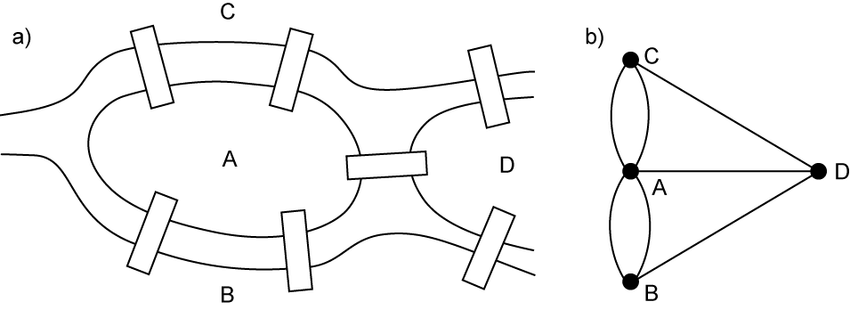
\includegraphics[width=0.4\textwidth]{../assets/konigsberg-bridges.png}
      \caption{The original seven bridges of Königsberg, which inspired Euler's work on graph theory.}
      \label{fig:konigsberg-bridges}
\end{figure}

\subsection{Early Graph Applications in AI}

In the early days of AI, graphs were primarily used to represent knowledge, relationships and reasoning.
Early AI pioneers like Marvin Minsky and others introduced \textbf{semantic networks} (graph-based knowledge representations) in the 1960s and 1970s to encode relationships between concepts in natural language understanding \cite{kelemen2007neural}.

Around the same time, probabilistic graphical models were developed - \textbf{Bayesian networks} introduced by Judea Pearl in the 1980s \cite{pearl1995bayesian} and \textbf{Markov random fields} \cite{lang2024abstract} - which leveraged graph structures (directed or undirected graphs) to represent probabilistic dependencies among variables for AI reasoning using joint \textbf{probability distributions} and \textbf{factor graphs} \cite{loeliger2004factor}.

These early uses of graphs in AI, however, treated graphs as static structures or as a backdrop for algorithms; there was \textit{no concept} of learning on graphs with neural networks yet.

% photo of Bayesian networks and Markov random fields
\begin{figure}[ht]
      \centering
      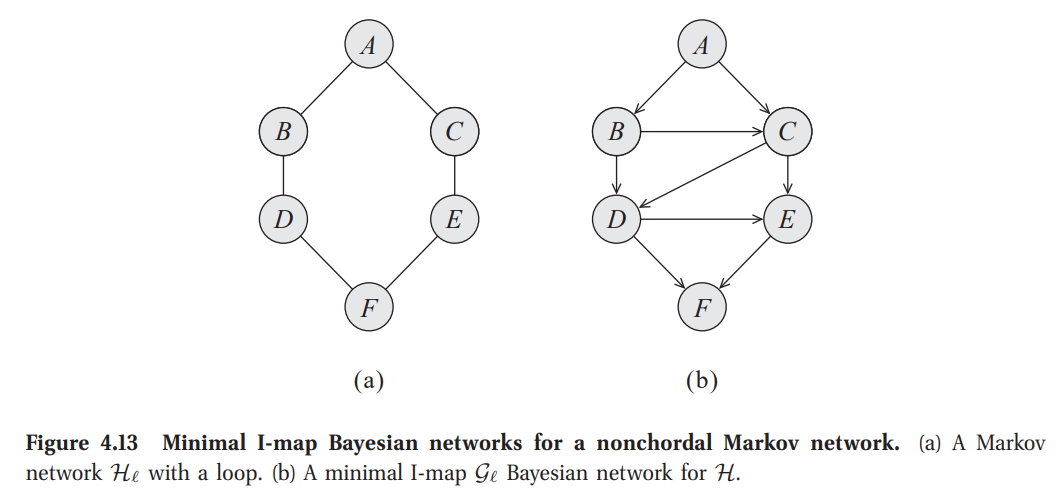
\includegraphics[width=1\textwidth,trim=0 100 0 0,clip]{../assets/bayesian-and-markov-networks.png}
      \caption{\textbf{Minimal I-map Bayesian networks for a nonchordal Markov network.} \\ (a) A Markov network $\mathcal{H}_\ell$ with a loop. (b) A minimal I-map $\mathcal{G}_\ell$ Bayesian network for $\mathcal{H}_\ell$.}
      \label{fig:bayesian-networks}
\end{figure}

\subsection{The Emergence of Graph Neural Networks}

The idea of combining neural networks with graph-structured data began to take shape in the 1990s.
Researchers explored recursive neural networks (RNNs) \cite{schmidt2019recurrent} and other architectures that could process structured inputs like sequences or trees.
Notably, Frasconi, Gori, and Sperduti (1998) \cite{frasconi1998general} proposed a \textbf{general framework} for adapting neural networks to structured data like graphs.
These early approaches could handle specific cases (often restricted to trees or acyclic graphs) by \textbf{recursively propagating information}, but they were \textit{limited} in scope and difficult to train.

A milestone was reached in 2007, when \textbf{Marco Gori} and colleagues introduced \textit{a new model for learning in graph domains} \cite{gori2007new} - essentially the first design of what we now call a \textbf{Graph Neural Network (GNN)}.

This was followed by \textit{Franco Scarselli}, \textit{Marco Gori}, and others formally defining the Graph Neural Network (GNN) model in 2009 \cite{scarselli2009graph}.
Scarselli et al.'s GNN was a neural network architecture that could directly take a graph as input and perform inference either at the node level or graph level, by iteratively propagating "state" information along the graph's edges until reaching a stable equilibrium.
This model extended earlier recursive neural net ideas and incorporated concepts from \textbf{random walks} and \textbf{Markov chains} on graphs.

In short, the GNN model of 2009 provided a way to learn node representations by an iterative \textbf{message-passing process} on the graph \cite{rizvi2022fimp}.
Early applications of these first GNNs included predicting properties of chemical compounds, classifying web pages (by modeling the web as a graph), fraud detection and other relational tasks.
The field was thus born from a marriage of graph theory (to represent relational structure) and neural network learning.

% photo of GNN message passing
\begin{figure}[ht]
      \centering
      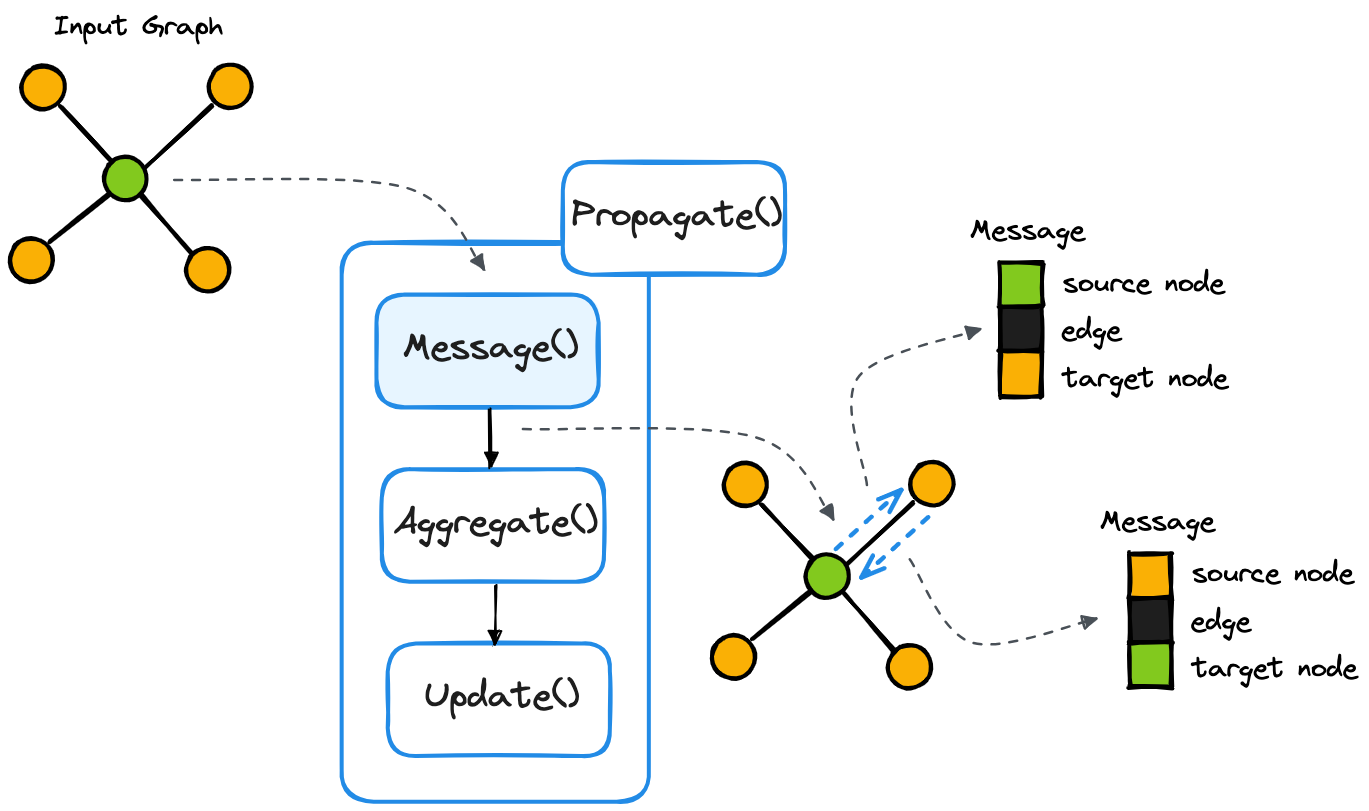
\includegraphics[width=0.8\textwidth]{../assets/gnn-message-passing.png}
      \caption{Message passing in Graph Neural Networks (GNNs).
            The GNN iteratively updates node representations by aggregating information from neighboring nodes, allowing it to learn complex relationships in graph-structured data.}
      \label{fig:gnn-message-passing}
\end{figure}

\section{Timeline of Key Developments in Graph Neural Networks}

From those initial ideas in 2005-2009, the area of graph-based neural networks has rapidly evolved.
Below is a timeline of major developments balancing historical milestones with recent advances:

\begin{itemize}
      \item \textbf{1736:} Euler solves the Königsberg bridge problem, laying the foundation for graph theory \cite{carlson2019konigsberg}. (While not AI, this marks the origin of graph theory itself).
      \item \textbf{1950s-1970s:} Graphs used in early AI knowledge representation (semantic networks) and problem-solving (state-space graphs for search algorithms). Marvin Minsky and others promote graph-based representations for AI knowledge \cite{kelemen2007neural}.
      \item \textbf{1980s:} Judea Pearl publishes \textit{Probabilistic Reasoning in Intelligent Systems}, introducing Bayesian networks (directed acyclic graphs) for AI reasoning \cite{pearl1995bayesian}. Markov random fields also emerge as undirected graphical models \cite{lang2024abstract}. Graphical models become a core AI tool (though not neural networks, they highlight the power of graphs in AI).
      \item \textbf{1997-1998:} Researchers (e.g. Goller \& Küchler; Frasconi, Gori \& Sperduti) propose neural network models for structured data such as trees and small graphs. These can be seen as precursors to modern GNNs. \cite{frasconi1998general}.
      \item \textbf{2007:} Gori, Monfardini, and Scarselli introduce the concept of a trainable neural network model for graphs \cite{gori2007new}. Also, they demonstrate GNNs for web page ranking and other tasks, showing that neural networks can learn on graph data (this is among the first uses of the term “Graph Neural Network”).
      \item \textbf{2009:} \textbf{Scarselli et al.} formally define \textbf{Graph Neural Networks (GNNs)} as a neural network architecture for graphs \cite{scarselli2009graph}. This paper formalizes GNNs and presents a learning algorithm for node- and graph-focused tasks. They prove that their GNN model has a form of universal approximation capability on graphs (under certain conditions) \cite{scarselli2009computational}, meaning it can represent a broad class of graph functions. However, training these early GNNs required an expensive iterative procedure (essentially performing graph recurrent neural network updates until convergence), which made them hard to scale to large or complex graphs.
      \item \textbf{2012:} \textbf{Krizhevsky et al.} introduce deep \textbf{convolutional neural networks (CNNs)} for image classification, achieving breakthrough performance on the ImageNet dataset \cite{krizhevsky2012imagenet}. This work popularizes deep learning and inspires subsequent research on graph-based deep learning methods.
      \item \textbf{2013:} The deep learning era meets graphs: Bruna et al. propose the first \textbf{graph convolutional network model} using spectral graph theory \cite{bruna2013spectral}. This approach generalizes convolutional neural networks (CNNs) from grid data (images) to graph data by working in the spectral domain of the graph Laplacian. This is a significant step in bridging deep learning with graph structures.
      \item \textbf{2014-2017:} Various advancements refine graph convolution. Notably, \textbf{Kipf \& Welling (2016)} introduce the \textbf{Graph Convolutional Network (GCN)}, which simplifies spectral convolutions to a very efficient form for semi-supervised learning on graphs \cite{kipf2017semigcn}. The GCN model operates in the spatial domain by a simple rule: each node iteratively aggregates (sums/averages) feature information from its neighbors and then applies a weight transformation. In \textbf{2017, Petar Veličković} et al. introduced \textbf{Graph Attention Networks (GATs)}, which extend GCNs by incorporating attention mechanisms to weigh neighbor contributions dynamically \cite{veličković2018graphattentionnetworks}. This allows GATs to learn which neighbors are most important for each node, improving performance on heterogeneous graphs.
      \item \textbf{2020-present:} GNNs become one of the hottest areas in deep learning research. Frameworks like \textbf{PyTorch Geometric} \cite{pytorch_geometric} and \textbf{DGL (Deep Graph Library)} \cite{dgl} are released to facilitate GNN development.

\end{itemize}

Researchers push GNNs into new domains: \textbf{graph transformers} emerge, combining transformers with graph structures for higher expressive power;
\textbf{hypergraph neural networks} handle hyperedges;
and \textbf{topological deep learning} blends graph neural nets with algebraic topology.
By 2021-2022, questions arose about the fundamental limits of message-passing GNNs. It remains an \textbf{open question} whether architectures strictly more powerful than message passing exist or whether any graph neural network can be reduced to message passing on some augmented graph.

In other words, researchers are debating how to go \textbf{beyond message-passing}, which currently underlies most GNN models.
Despite this, the impact of GNNs is undeniable - they achieved breakthroughs like deep learning on molecules, predicting protein structures, and powerfully modeling relational data across disciplines.

This essay examines the \textbf{fundamental concepts} and \textbf{core applications} of Graph Neural Networks, providing a comprehensive analysis of their theoretical foundations rather than surveying recent research developments.
Building upon the foundational 2009 GNN model discussed above, we proceed to analyze the \textbf{Graph Convolutional Network (GCN)} architecture, establishing theoretical and practical comparisons with \textbf{Convolutional Neural Networks (CNNs)}. Subsequently, we investigate \textbf{Graph Attention Networks (GATs)}, which represent a significant advancement in GNN design through the incorporation of attention mechanisms that enable dynamic weighting of neighboring node contributions.

\section{Convolutional Neural Networks and Graph Convolutional Networks}

\textbf{Convolutional Neural Networks (CNNs)} \cite{krizhevsky2012imagenet} have revolutionized the field of computer vision by leveraging the spatial structure of images.
An image is like a grid of pixels. A CNN looks at small parts of the grid at a time.
They apply convolutional filters to these local regions of the input image, allowing them to learn hierarchical features and patterns.
Then the network uses these patterns to find more complex shapes. CNNs use many layers of filters. Each layer finds more detailed features.
This approach has led to significant advancements in image classification, object detection, and segmentation tasks.

% break the page
\newpage

% photo of CNN architecture
\begin{figure}[h]
      \centering
      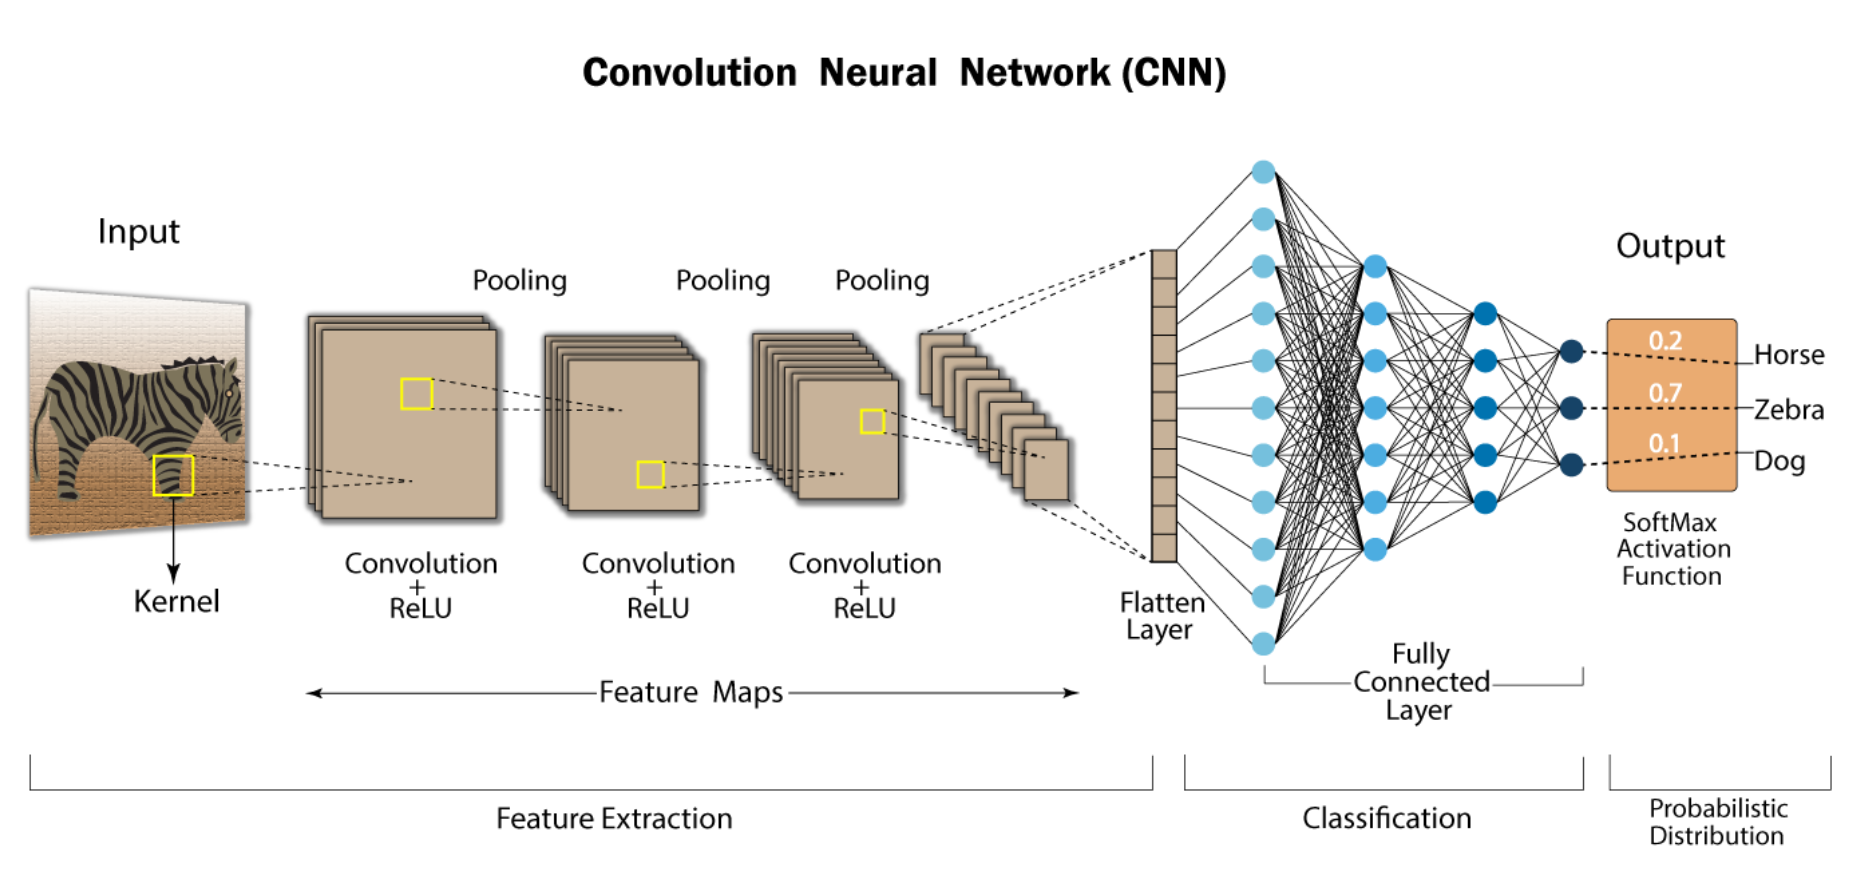
\includegraphics[width=1.0\textwidth]{../assets/cnn_architecture.png}
      \caption{A typical Convolutional Neural Network (CNN) architecture, which applies convolutional filters (layers) to learn hierarchical features from image.}
      \label{fig:cnn-architecture}
\end{figure}

\textbf{Graph Convolutional Networks (GCNs)}, on the other hand, extend the principles of CNNs to graph-structured data.
In a GCN, the convolution operation is defined in terms of the graph's topology, enabling the model to capture relationships between nodes and their neighbors.

\vspace{0.9cm}

\textbf{How does it work?}

A standard GCN layer operates through the following steps for each node $i$ in the graph:

\begin{enumerate}
    \item \textbf{Gather Features:} Collect the current feature vectors $h_j$ from all neighbors $j \in \mathcal{N}(i)$, plus the node's own feature $h_i$.
    
    \item \textbf{Normalize:} Because nodes have different degrees (numbers of neighbors), GCNs use a normalization factor. A common choice following \textbf{Kipf \& Welling (2016)} \cite{kipf2017semigcn} is:
    \begin{equation}
        \tilde{A} = A + I, \quad D_i = \sum_j \tilde{A}_{ij}, \quad \text{so that } D^{-\frac{1}{2}} \tilde{A} D^{-\frac{1}{2}}
    \end{equation}
    where $A$ is the adjacency matrix and $I$ adds self-loops. This ensures each neighbor's contribution is scaled appropriately.
    
    \item \textbf{Apply Shared Weights:} Multiply the stack of gathered and normalized features by a weight matrix $W$. This transforms the aggregated neighborhood information into a new feature space.
    
    \item \textbf{Nonlinearity:} Pass the result through an activation function like ReLU (i.e., $\max(0, \cdot)$) to introduce non-linear modeling capabilities.
\end{enumerate}

Putting it all together, one \textbf{standard GCN layer} updates the node feature matrix $H$ as:
\begin{equation}
    H^{(k+1)} = \sigma\left(D^{-\frac{1}{2}} \tilde{A} D^{-\frac{1}{2}} H^{(k)} W^{(k)}\right),
\end{equation}
where:
\begin{itemize}
    \item $H^{(k)}$ is the matrix of node features at layer $k$
    \item $W^{(k)}$ is the learnable weight matrix for layer $k$
    \item $\sigma$ is an activation (e.g., ReLU)
    \item $D^{-\frac{1}{2}} \tilde{A} D^{-\frac{1}{2}}$ smoothly averages each node's neighbors (including itself) before applying $W$
\end{itemize}

% photo of GCN architecture
\begin{figure}[h]
      \centering
      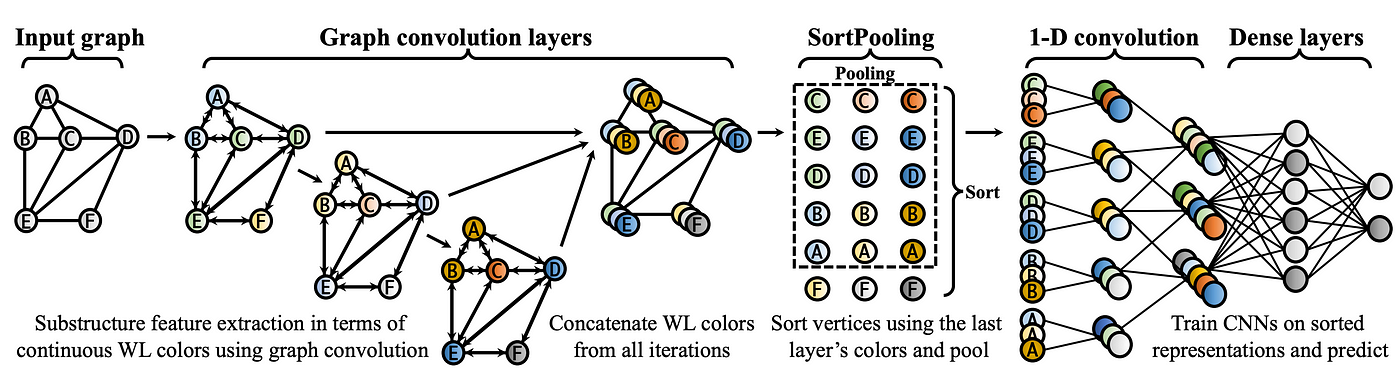
\includegraphics[width=1.0\textwidth]{../assets/gcn_architecture.png}
      \caption{A typical Graph Convolutional Network (GCN) architecture. The input graph undergoes multiple graph convolution layers that aggregate neighborhood features using graph convolution operations. Each layer transforms node features through message passing, followed by sort pooling to create a fixed-size representation, 1-D convolution for pattern extraction, and dense layers for final prediction. Colors in nodes represent different feature embeddings learned at each layer.}
      \label{fig:gcn-architecture}
\end{figure}

By stacking multiple GCN layers, each node learns from nodes that are progressively farther away in the graph, enabling the capture of long-range dependencies and complex structural patterns.

This is particularly useful for tasks such as node classification, link prediction, and graph classification.

Both CNNs and GCNs share a common goal: to learn meaningful representations from structured data.
However, they differ in their underlying assumptions and the types of relationships they can model.
While CNNs excel at capturing local patterns in grid-like data, GCNs are designed to handle the irregular and complex structures found in graphs.
In GCNs each node's new feature is influenced by its neighbors. Over multiple layers, information flows farther out (2 hops, 3 hops, $\dots$), letting each node gather context from a wider subgraph.
Also, unlike fully-connected layers, GCNs use one weight matrix $W$ per layer for all nodes—scaling gracefully to large graphs. Thus, they can efficiently process large graphs without a combinatorial explosion in parameters.


\bibliographystyle{unsrt}
\bibliography{references}

\end{document}
